\documentclass{article}

\usepackage[margin=1in]{geometry}
\usepackage{parskip}
\usepackage{graphicx}

\usepackage{tikz}

\usepackage{listings}
\lstset{
  basicstyle=\ttfamily\small,
  breaklines=true,
  frame=single
}
\usepackage{physics}
\usepackage{amsmath}
\usepackage{amssymb}
\usepackage{hyperref}
\hypersetup{
  colorlinks=true,
  linkcolor=blue,
  filecolor=magenta,
  urlcolor=cyan,
  pdftitle={INTDER Manual},
  pdfpagemode=FullScreen,
}

\title{Rust INTDER Manual}
\date{}
\author{Brent R. Westbrook}

\begin{document}

\maketitle

INTDER is a program for performing coordinate transformations between
simple-/symmetry-internal coordinates and Cartesian coordinates. It was
originally written in Fortran by Wesley D. Allen and coworkers but has since
been translated to Rust by Brent R. Westbrook. This documentation corresponds to
the Rust version only.

\section{Internal Coordinates}
\label{sec:coords}

At their most basic, internal coordinates are those defined with reference to
other atoms in the same molecule (or system), as opposed to an external set of
axes or some other frame of reference. Simple examples of internal coordinates
are distances between pairs of atoms and angles between sets of three atoms. A
major benefit of using internal coordinates over an external coordinate system
like Cartesian coordinates is that internal coordinates require only 3$N-6$ (or
3$N-5$ for linear molecules) coordinates to describe a system fully since the 3
translational and 3 rotational degrees of freedom only have meaning in an
external reference frame. $N$ in this case is, of course, the number of atoms in
the system. Given the exponential scaling of the number of points required to
describe a quartic force field (QFF), or really any potential energy surface
(PES), with the number atoms, this difference of 6 coordinates can have a large
effect. As a result, using internal coordinates can lead to a substantial
decrease in computational cost for such a PES. The types of simple-internal
coordinates supported by INTDER are described in the following subsections.

\subsection{Simple-Internal Coordinates}
\label{sec:simple}

\subsubsection{Stretch}
\label{sec:stretch}

The bond stretch, referred to as \verb|STRE| in the input file, is the distance
between two atoms, as shown in Fig.~\ref{fig:stre}. When the direction matters,
the distance is computed from atom \verb|A| to atom \verb|B|, using the equation
given in Eqn.~\ref{eq:stre}, where $a_i$ and $b_i$ represent the $i$th
components of the Cartesian coordinates of atoms \verb|A| and \verb|B|,
respectively.

\begin{figure}[ht]
  \centering
  \caption{A stretch}
  \label{fig:stre}

  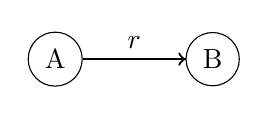
\begin{tikzpicture}
    \node[draw,circle] (A) at (0,0) {A};
    \node[draw,circle] (B) at (2,0) {B};
    \draw[thick, ->] (A) to (B);
    \draw[thick] (A) -- (B) node[midway, above] {$r$};
  \end{tikzpicture}
\end{figure}

\begin{equation}
  \label{eq:stre}
  r = \sqrt{\sum_i (b_i - a_i)^2}
\end{equation}

\subsubsection{Bend}
\label{sec:bend}

The bend, referred to as \verb|BEND| in the input file, is the angle between
three atoms, as shown in Fig.~\ref{fig:bend}.

\begin{figure}[ht]
  \centering
  \caption{A bend}
  \label{fig:bend}

  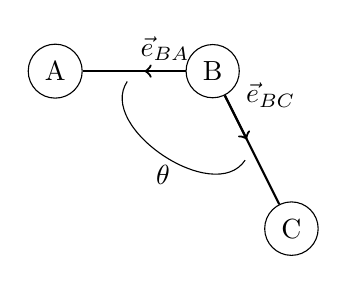
\begin{tikzpicture}
    \node[draw,circle] (A) at (0,0) {A};
    \node[draw,circle] (B) at (2,0) {B};
    \node[draw,circle] (C) at (3,-2) {C};
    \draw[thick] (A) -- (B) node[midway] (m) {};
    \draw[thick] (B) -- (C) node[midway] (n) {};
    \path (m) edge [bend left=-90] node[below] {$\theta$} (n);
    \draw[thick, ->] (B) -- (m) node[midway, above] {$\vec{e}_{BA}$};
    \draw[thick, ->] (B) -- (n) node[midway, above right] {$\vec{e}_{BC}$};
  \end{tikzpicture}
\end{figure}

The value of the angle, $\theta$ is computed using Eqn.~\ref{eq:bend}, where
$\vec{e}_{ij}$ represents the unit vector pointing from atom $i$ to atom $j$.

\begin{equation}
  \label{eq:bend}
  \theta = \acos(\vec{e}_{BA} \cdot \vec{e}_{BC})
\end{equation}

\subsubsection{Torsion}
\label{sec:tors}

The torsional angle, referred to as \verb|TORS| in the input file, is the angle
between the planes formed by the overlapping sets of atoms \verb|A|, \verb|B|,
\verb|C|, and \verb|B|, \verb|C|, \verb|D|, as shown in Fig.~\ref{fig:tors}.
Vectors $\vec{v}_5$ and $\vec{v}_6$ are the vectors normal to the planes $ABC$
and $BCD$, respectively, found by $\vec{e}_{BA} \times \vec{e}_{CB}$ and
$\vec{e}_{DC} \times \vec{e}_{CB}$. To find the angle $\theta$ between these two
normals, and thus between the planes, perform the following transformations:

\begin{align}
  w_2 &= \vec{e}_{BA} \cdot \vec{e}_{CB} \\
  w_3 &= \vec{e}_{DC} \cdot \vec{e}_{CB} \\
  s_2 &= \sqrt{1 - w_2^2} \\
  s_3 &= \sqrt{1 - w_3^2} \\
  w_4 &= \vec{e}_{BA} \cdot \vec{v}_{6} \\
  w_5 &= -\vec{v}_5 \cdot \vec{v}_6 \\
  w &= \frac{w_2}{s_2 s_3} \\
  \theta_0 &= \asin w \\
  \theta &= \begin{cases}
              \theta_0 & w_3 \geq 0 \\
              \pi - \theta_0 & w_3 < 0
            \end{cases}
\end{align}

\begin{figure}[ht]
  \centering
  \caption{A torsion}
  \label{fig:tors}

  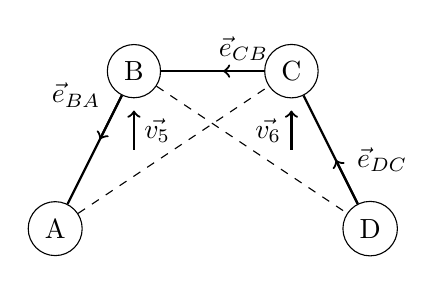
\begin{tikzpicture}
    \node[draw,circle] (B) at (0,0) {B};
    \node[draw,circle] (C) at (2,0) {C};
    \node[draw,circle] (D) at (3,-2) {D};
    \node[draw,circle] (A) at (-1,-2) {A};
    \draw[thick] (B) -- (A) node[midway] (m) {};
    \draw[thick] (C) -- (B) node[midway] (n) {};
    \draw[thick] (D) -- (C) node[midway] (o) {};
    \draw[thick, ->] (B) -- (m) node[midway, above left] {$\vec{e}_{BA}$};
    \draw[thick, ->] (C) -- (n) node[midway, above] {$\vec{e}_{CB}$};
    \draw[thick, ->] (D) -- (o) node[midway, above right] {$\vec{e}_{DC}$};
    % vectors
    \draw[thick, ->] (0,-1) -- (0,-0.5) node[midway, right] {$\vec{v_5}$};
    \draw[thick, ->] (2,-1) -- (2,-0.5) node[midway, left] {$\vec{v_6}$};
    % planes
    \draw[dashed] (A) -- (C);
    \draw[dashed] (B) -- (D);
  \end{tikzpicture}
\end{figure}

\subsubsection{Lin1}
\label{sec:lin1}

TODO

\subsubsection{Out}
\label{sec:out}

TODO

\end{document}